\documentclass[tikz,convert={outfile=\jobname.svg}]{standalone}
%\usetikzlibrary{...}% tikz package already loaded by 'tikz' option
\begin{document}
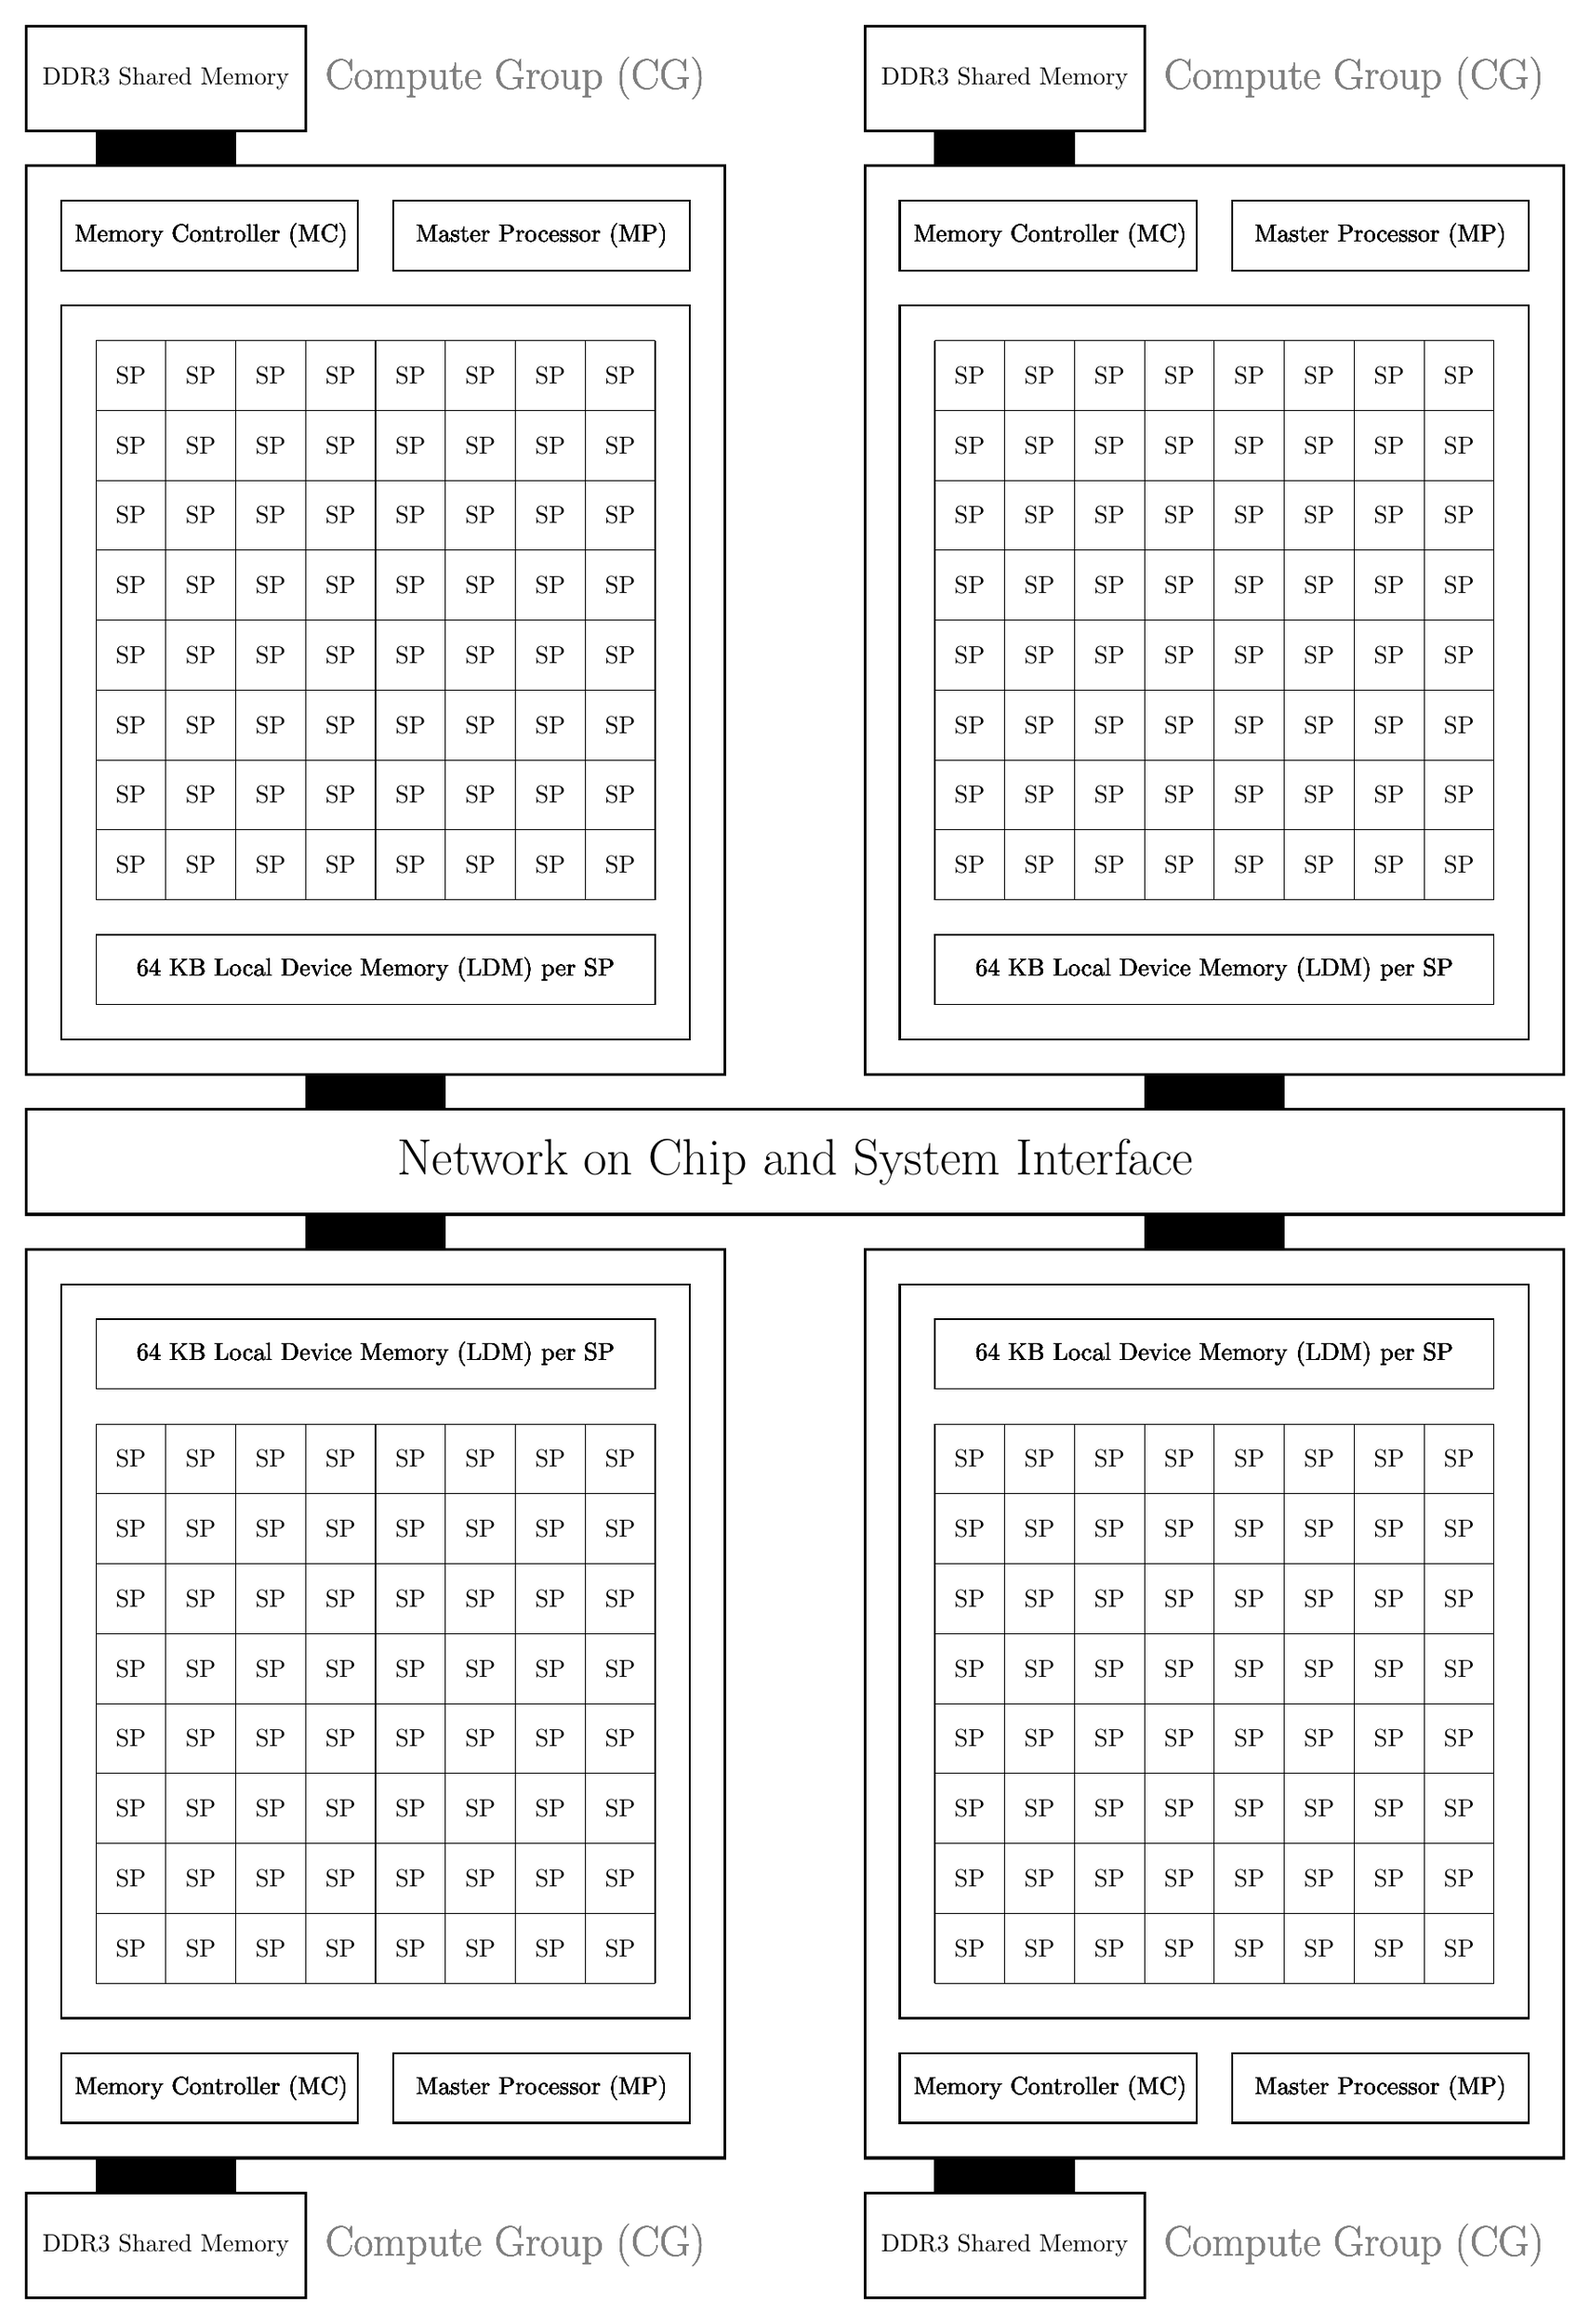
\begin{tikzpicture}% Example:

\foreach \off in {0, 12} {
\begin{scope}[shift={(\off, 0)}]

\draw (0,0) grid (8,8);

% SPs
\draw[thick] (-0.5, -2) rectangle (8.5, 8.5);
\foreach \i in {0, 1, 2, 3, 4, 5, 6, 7} {
    \foreach \j in {0, 1, 2, 3, 4, 5, 6, 7} {
        \draw (\i+0.5, \j+0.5) node[auto]{SP};    
    }
\draw (0, -1.5) rectangle (8, -0.5);
\draw (4, -1.0) node[auto] {64 KB Local Device Memory (LDM) per SP};
    
% CG
\draw[very thick] (-1, -2.5) rectangle (9, 10.5);
\begin{LARGE}
\draw[color=black!50] (6, 11.75) node[auto] {Compute Group (CG)};
\end{LARGE}

% MC
\draw[thick] (-0.5, 9) rectangle (3.75, 10);
\draw (1.65, 9.5) node[auto] {Memory Controller (MC)};

% MP
\draw[thick] (4.25, 9) rectangle (8.5, 10);
\draw (6.375, 9.5) node[auto]{Master Processor (MP)};
}

% RAM
\draw [very thick] (-1, 11) rectangle (3, 12.5);
\draw (1, 11.75) node[auto] {DDR3 Shared Memory};
\draw[fill] (0, 10.5) rectangle (2, 11);

\end{scope}
}

\foreach \off in {0, 12} {
\begin{scope}[shift={(\off, -15.5)}]


\draw (0,0) grid (8,8);

% SPs
\draw[thick] (-0.5, -2+1.5) rectangle (8.5, 8.5+1.5);
\foreach \i in {0, 1, 2, 3, 4, 5, 6, 7} {
    \foreach \j in {0, 1, 2, 3, 4, 5, 6, 7} {
        \draw (\i+0.5, \j+0.5) node[auto]{SP};    
    }
\draw (0, -1.5+10) rectangle (8, -0.5+10);
\draw (4, -1.0+10) node[auto] {64 KB Local Device Memory (LDM) per SP};


% CG
\draw[very thick] (-1, -2.5) rectangle (9, 10.5);
\begin{LARGE}
\draw[color=black!50] (6, 11.75-15.5) node[auto] {Compute Group (CG)};
\end{LARGE}

% MC
\draw[thick] (-0.5, 9-11) rectangle (3.75, 10-11);
\draw (1.65, 9.5-11) node[auto] {Memory Controller (MC)};

% MP
\draw[thick] (4.25, 9-11) rectangle (8.5, 10-11);
\draw (6.375, 9.5-11) node[auto]{Master Processor (MP)};
}

% RAM
\draw [very thick] (-1, 11-15.5) rectangle (3, 12.5-15.5);
\draw (1, 11.75-15.5) node[auto] {DDR3 Shared Memory};
\draw[fill] (0, 10.5-13.5) rectangle (2, 11-13.5);

\end{scope}
}

% NOC
\draw[very thick] (-1, -4.5) rectangle (21, -3);
\begin{huge}
\draw (10, -3.75) node[auto] {Network on Chip and System Interface};
\end{huge}

\foreach \i in {0, 1} {
    \foreach \j in {0, 1} {
         \draw[fill] (3+\i*12, -2.5-\j*2) rectangle (5+\i*12, -3-\j*2); 
    }
}

\end{tikzpicture}
\end{document}